\ylDisplay{Voltmeeter} % Ülesande nimi
{Erkki Tempel} % Autor
{piirkonnavoor} % Voor
{2017} % Aasta
{G 1} % Ülesande nr.
{1} % Raskustase
{
% Teema: Elektriahelad
\ifStatement
Joonisel näidatud elektriskeemis on ideaalne ampermeeter, mis näitab voolutugevust $I$. Ampermeeter asendatakse ideaalse voltmeetriga. Kui suur on voltmeetri näit? Kõikide takistite takistus on $R$.
\begin{center}
	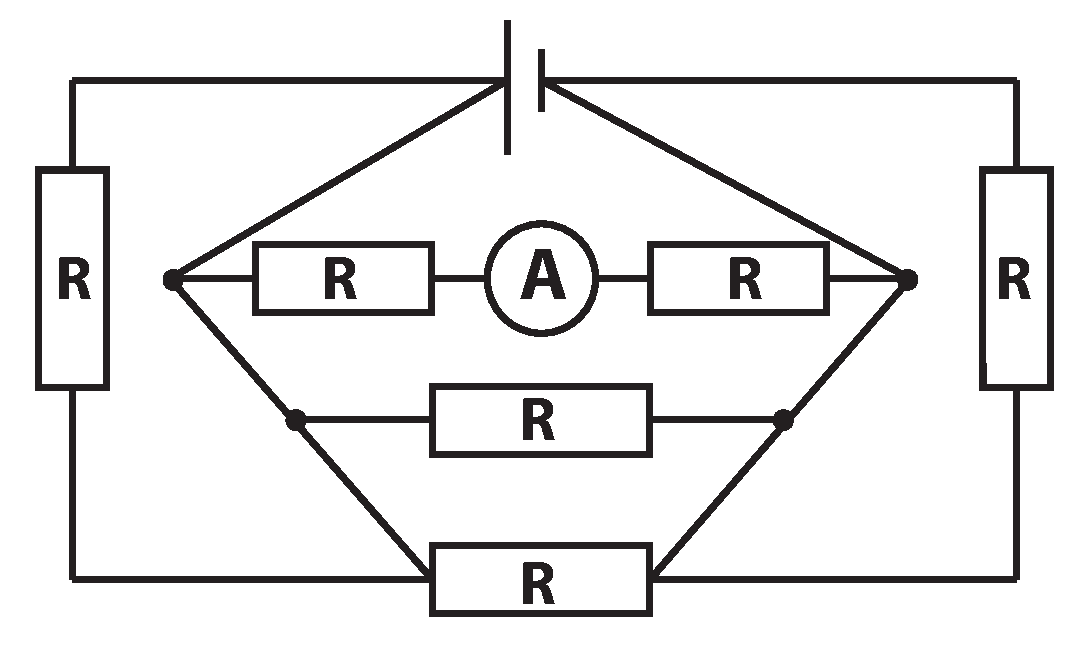
\includegraphics[width=0.4\textwidth]{2017-v2g-01-skeem}
\end{center}
\fi


\ifHint
Jooniselt näeme, et äärmised takistid on lühistatud, mistõttu need mõõteriistade näitu ei mõjuta.
\fi


\ifSolution
Jooniselt näeme, et äärmised takistid on lühistatud, mistõttu need mõõteriistade näitu ei mõjuta. Ampermeeter on jadamisi kahe takistiga, mistõttu on ampermeetriga harus kogutakistus $2R$. Seega on kogupinge selles harus võrdne patarei pingega
\[ U = I\cdot 2R.\]
Asendades ampermeetri voltmeetriga, näitab voltmeeter patarei pinget, kuna tegemist on ideaalse voltmeetriga, mille takistus on lõpmatu. Sellest tulenevalt voltmeetriga haru vool ei läbi ja temaga jadamisi ühendatud takistid voltmeetri näitu ei mõjuta.

\[ U\idx{voltmeeter} = 2RI.\]
\fi


\ifEngStatement
% Problem name: Voltmeter
In the circuit diagram pictured below there is an ideal ammeter which shows a current $I$. The ammeter is replaced by an ideal voltmeter. How big is the voltmeter’s reading? The resistance of all the resistors is $R$.
\begin{center}
	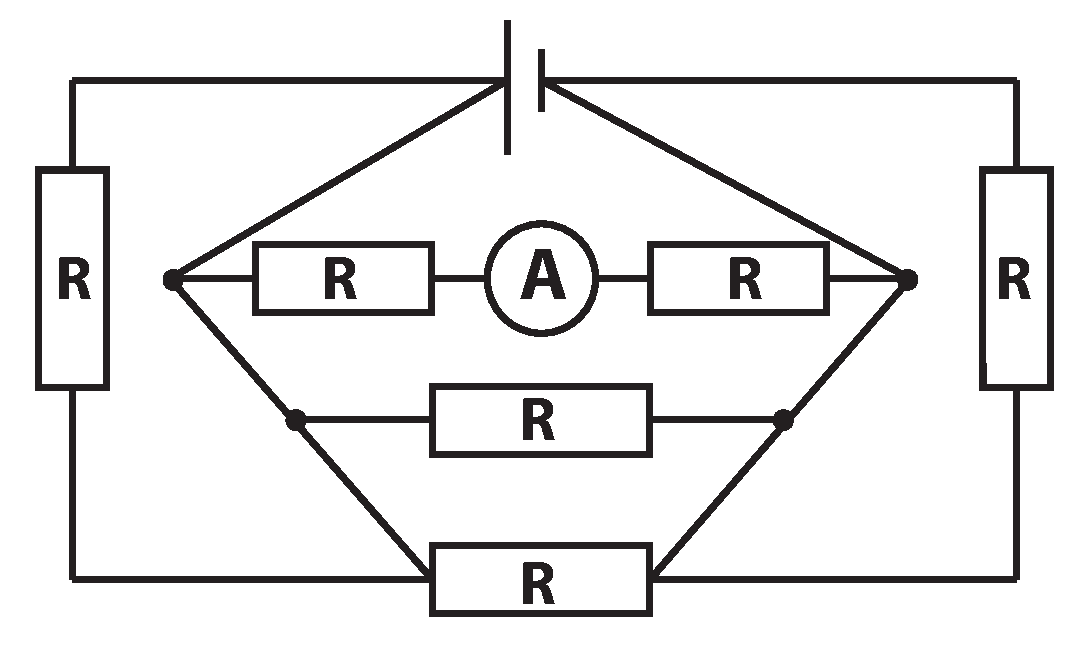
\includegraphics[width=0.4\textwidth]{2017-v2g-01-skeem}
\end{center}
\fi


\ifEngHint
We can see from the figure that the outer resistors are short-circuited which is why they do not affect the reading of the measurement devices.
\fi


\ifEngSolution
From the figure we see that the outer resistors are short-circuited which is why they do not affect the readings of the measuring instruments. The ammeter is connected in series to two resistors which is why the total resistance is $2R$ in the branch with the ammeter. Therefore the total voltage in the branch is equal to the voltage of the battery
\[ U = I\cdot 2R.\] 
If we replace the ammeter with a voltmeter then the voltmeter will show the battery’s voltage, because we are dealing with an ideal voltmeter that has an infinite resistance. Because of this no current will go through the branch with the voltmeter and the resistors that are connected in series to the voltmeter do not affect the reading.
\[ U\idx{voltmeter} = 2RI.\]
\fi
}